\section{Simulation Analysis}
\label{sec:simulation}

\subsection{Operating point analysis for t$<$0}

In this section, an operating point analysis of the circuit (referência ao circuito) was conducted in order to calculate the voltage in all nodes and the current through the resistors for a t $<$ 0. To contextualize the values obtained using the tools in ngspice, it is necessary to state that, as node 0 is connected to ground, its nodal voltage does not appear on the table of results. It is important to note that an extra voltage source, Vaux, was added and therefore, another node was also added (node 9). This Vaux was intended to allow the measurement of the current Id which voltage source Vd depends on, since ngspice doesn't allow us to introduce Resistor R6's current in the computation. Vaux's voltage is equal to 0 V, since it is only an auxiliary component that doesn't interfere with the circuit (node's 7 voltage is equal to node's 9 voltage) and allowed us to obtain the current through it.

%Introduzir a primeira tabela dos valores das correntes e da tensão dos nós do spice e do octave lado a lado para comparar o erro
\begin{table}[h] 
\begin{minipage}{0.5\linewidth}
\centering
\begin{tabular}{|
>{\columncolor[HTML]{FFCC67}}l |c|}
\hline
\multicolumn{2}{|l|}{\cellcolor[HTML]{EABD8B}NgSpice - Voltages (V)} \\ \hline
@cb[i] & 0.000000e+00\\ \hline
@ce[i] & 0.000000e+00\\ \hline
@q1[ib] & 7.022567e-05\\ \hline
@q1[ic] & 1.404513e-02\\ \hline
@q1[ie] & -1.41154e-02\\ \hline
@q1[is] & 5.765392e-12\\ \hline
@rc[i] & 1.411536e-02\\ \hline
@re[i] & 1.411536e-02\\ \hline
@rf[i] & 7.022567e-05\\ \hline
@rs[i] & 0.000000e+00\\ \hline
v(1) & 0.000000e+00\\ \hline
v(2) & 0.000000e+00\\ \hline
base & 2.254108e+00\\ \hline
coll & 5.765392e+00\\ \hline
emit & 1.411536e+00\\ \hline
vcc & 1.000000e+01\\ \hline

\end{tabular}
\end{minipage}%
\begin{minipage}{0.5\linewidth}
\centering
\begin{tabular}{|
>{\columncolor[HTML]{FFCC67}}l |c|}
\hline
\multicolumn{2}{|l|}{\cellcolor[HTML]{EABD8B}Octave - Voltages (V)} \\ \hline
V1 & & 8.194795e+00 V\\ \hline
V2 & & 7.917828e+00 V\\ \hline
V3 & & 7.340169e+00 V\\ \hline
V4 & & 2.978754e+00 V\\ \hline
V5 & & 7.957540e+00 V\\ \hline
V6 & & 1.197664e+01 V\\ \hline
V7 & & 9.776608e-01 V\\ \hline
V8 & & 0.000000e+00 V\\ \hline

\end{tabular} 
\end{minipage}
\caption{Nodal Voltage Comparison}
\end{table}


\subsection{Calculus of $Req$ - Simulation}

Similarly to the last section, an operating point analysis to the circuit (referência ao circuito) was conducted, with the difference being that the voltage source $vs$ was turned off and the capacitor was replaced by the independent voltage source $Vx$ which corresponds to the value of $v(6)$-$v(8)$. This $Vx$ is equivalent to the voltage in the capacitor's terminals. 
The values of currents and nodal voltages were then put in a table, while the equivalent thevenin resistor was calculated by the following equation:

\begin{equation}
Req = (v(6)-v(8))/vxbranch,
\end{equation}
with $vxbranch$ corresponding to the current $Ix$ that flows through the $Vx$'s branch.

%Introduzir a primeira tabela dos valores das correntes e da tensão dos nós do spice e do octave lado a lado para comparar o erro
\begin{table}[h] 
\begin{minipage}{0.5\linewidth}
\centering
\begin{tabular}{|
>{\columncolor[HTML]{FFCC67}}l |c|}
\hline
\multicolumn{2}{|l|}{\cellcolor[HTML]{EABD8B}NgSpice - Voltages (V)} \\ \hline
@gb[i] & 0.000000e+00\\ \hline
@r1[i] & 0.000000e+00\\ \hline
@r2[i] & 0.000000e+00\\ \hline
@r3[i] & 0.000000e+00\\ \hline
@r4[i] & 0.000000e+00\\ \hline
@r5[i] & -1.63724e-02\\ \hline
@r6[i] & 0.000000e+00\\ \hline
@r7[i] & 0.000000e+00\\ \hline
v(1) & 0.000000e+00\\ \hline
v(2) & 0.000000e+00\\ \hline
v(3) & 0.000000e+00\\ \hline
v(5) & 0.000000e+00\\ \hline
v(6) & 5.000000e+01\\ \hline
v(7) & 0.000000e+00\\ \hline
v(8) & 0.000000e+00\\ \hline
v(9) & 0.000000e+00\\ \hline

\end{tabular}
\end{minipage}%
\begin{minipage}{0.5\linewidth}
\centering
\begin{tabular}{|
>{\columncolor[HTML]{FFCC67}}l |c|}
\hline
\multicolumn{2}{|l|}{\cellcolor[HTML]{EABD8B}Octave - Voltages (V)} \\ \hline
V1 & 0.000000e+00 V\\ \hline
V2 & -0.000000e+00 V\\ \hline
V3 & -0.000000e+00 V\\ \hline
V4 & -0.000000e+00 V\\ \hline
V5 & 0.000000e+00 V\\ \hline
V6 & 5.000000e+01 V\\ \hline
V7 & 0.000000e+00 V\\ \hline
V8 & -0.000000e+00 V\\ \hline

\end{tabular} 
\end{minipage}
\caption{Nodal Voltage Comparison}
\end{table}


\subsection{Transient Analysis for t $\geq$ (Natural Solution)}

In this section, a transient analysis was conducted in order to evaluate the natural response of the circuit, which means, the variation over time. Once that to calculate the natural response, the voltage source $vs$ is turned off, the circuit simulated was equal to the one in the previous question. From this, the voltage in the capacitor's over time (time interval considered was [0,20]ms) was calculated and plotted, using $Vx$ (calculated in the previous section) as the initial condition for the capacitor's voltage.

\begin{figure}[h] 
\centering
\begin{subfigure}{0.5\textwidth}
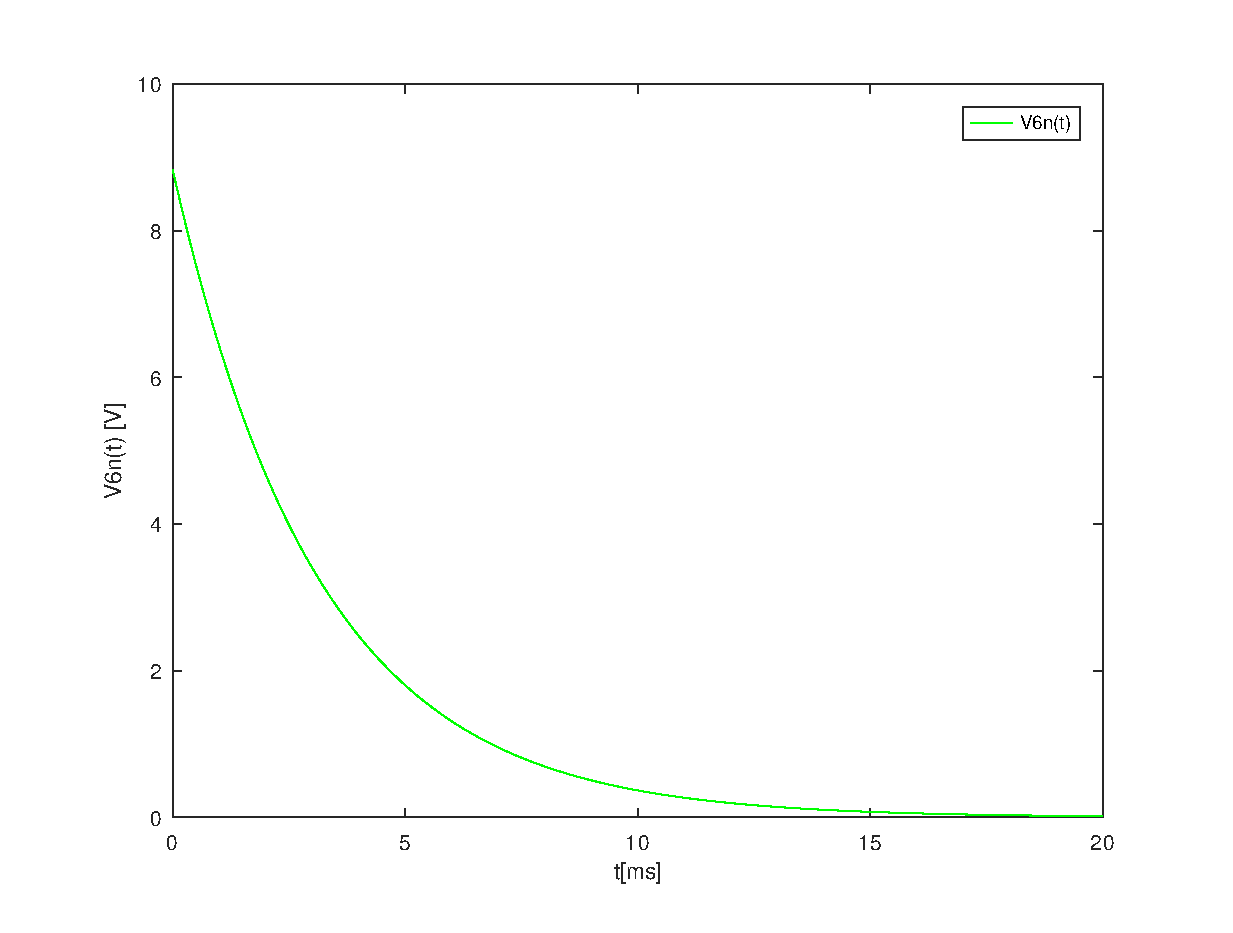
\includegraphics[width=\textwidth]{NaturalResponse.eps}
\caption{Natural Response (Octave)}
\label{fig:first}
\end{subfigure}
\begin{subfigure}{0.42\textwidth}
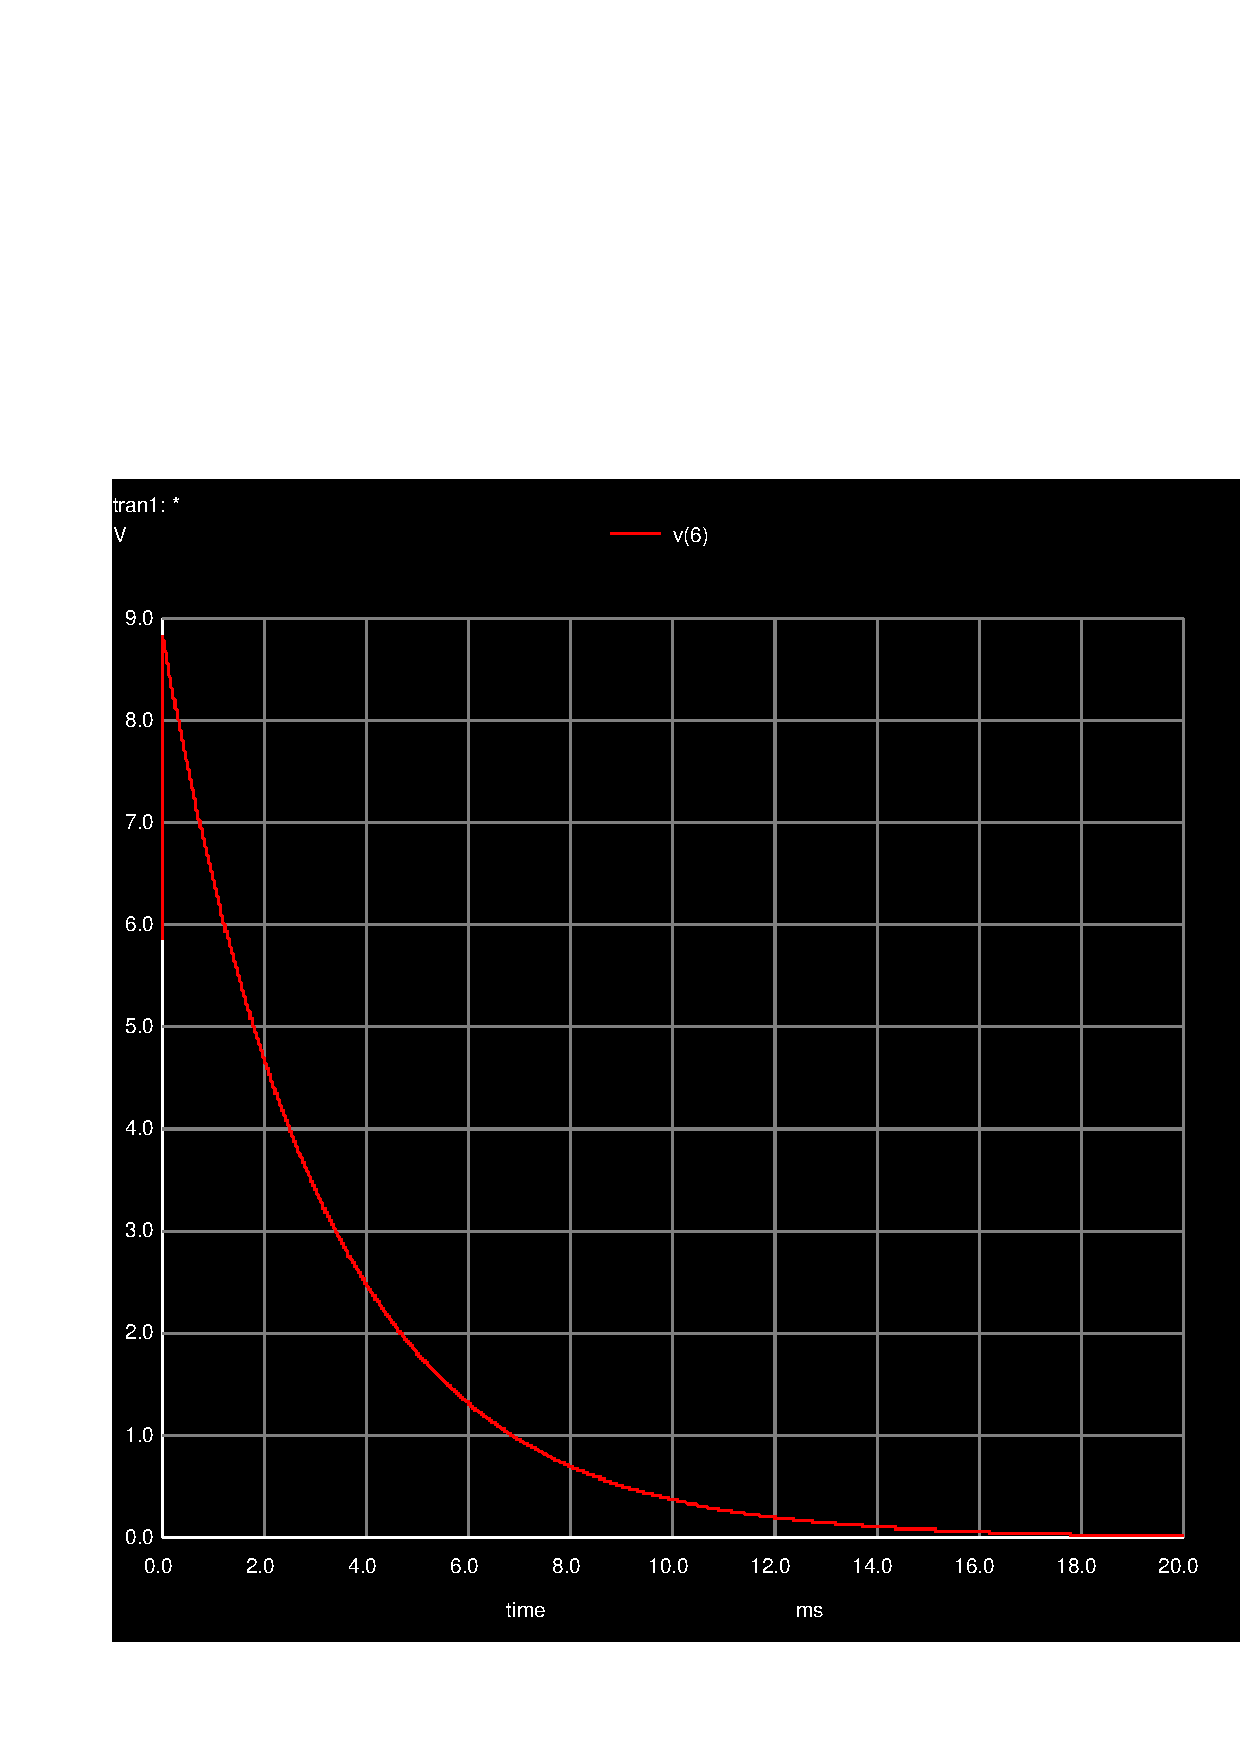
\includegraphics[width=\textwidth]{sim_3.pdf}
\caption{Natural Response (NGSpice)}
\label{fig:second}
\end{subfigure}
\end{figure}
 
 When observing the graph obtained from the simulation in Ngspice, we see that the capacitor's voltage overtime is a negative exponential matching the one obtained from the theorethical analysis in octave.
 
\pagebreak
 
\subsection{Operating Point Analysis for t $\geq$ (Natural and Forced Solution)}
In this section, as previously, a transient analysis was conducted in order to evaluate the natural and forced response of the circuit. In order to achieve this, the procedure adopted was the same as the one in the previous step, but with the voltage souce $vs(t)$ consisting of a sinusoidal wave sen(2*$\pi$*f).  

\begin{figure}[h] 
\centering
\begin{subfigure}{0.5\textwidth}
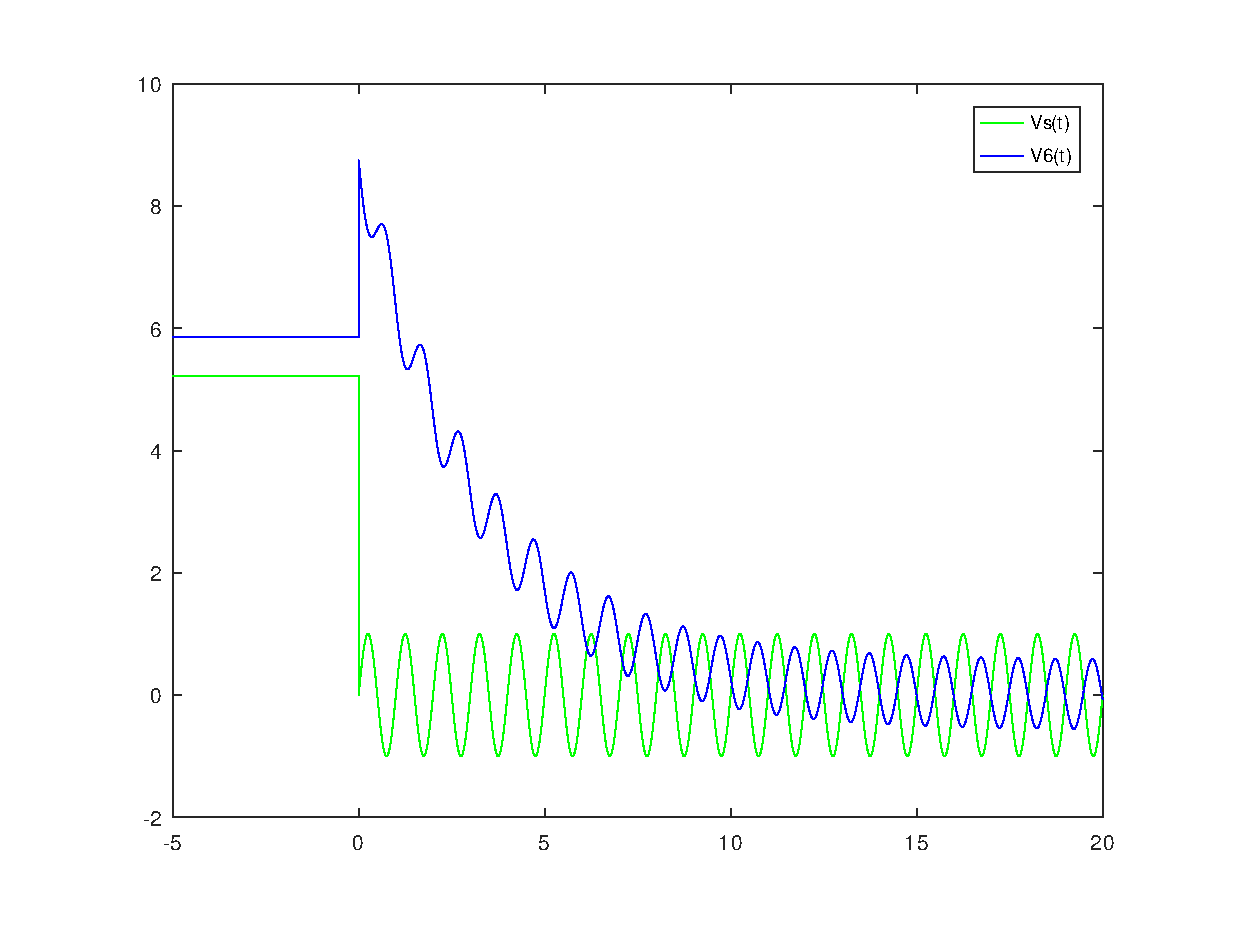
\includegraphics[width=\textwidth]{Solution.eps}
\caption{Natural and forced response (Octave)}
\label{fig:first}
\end{subfigure}
\begin{subfigure}{0.42\textwidth}
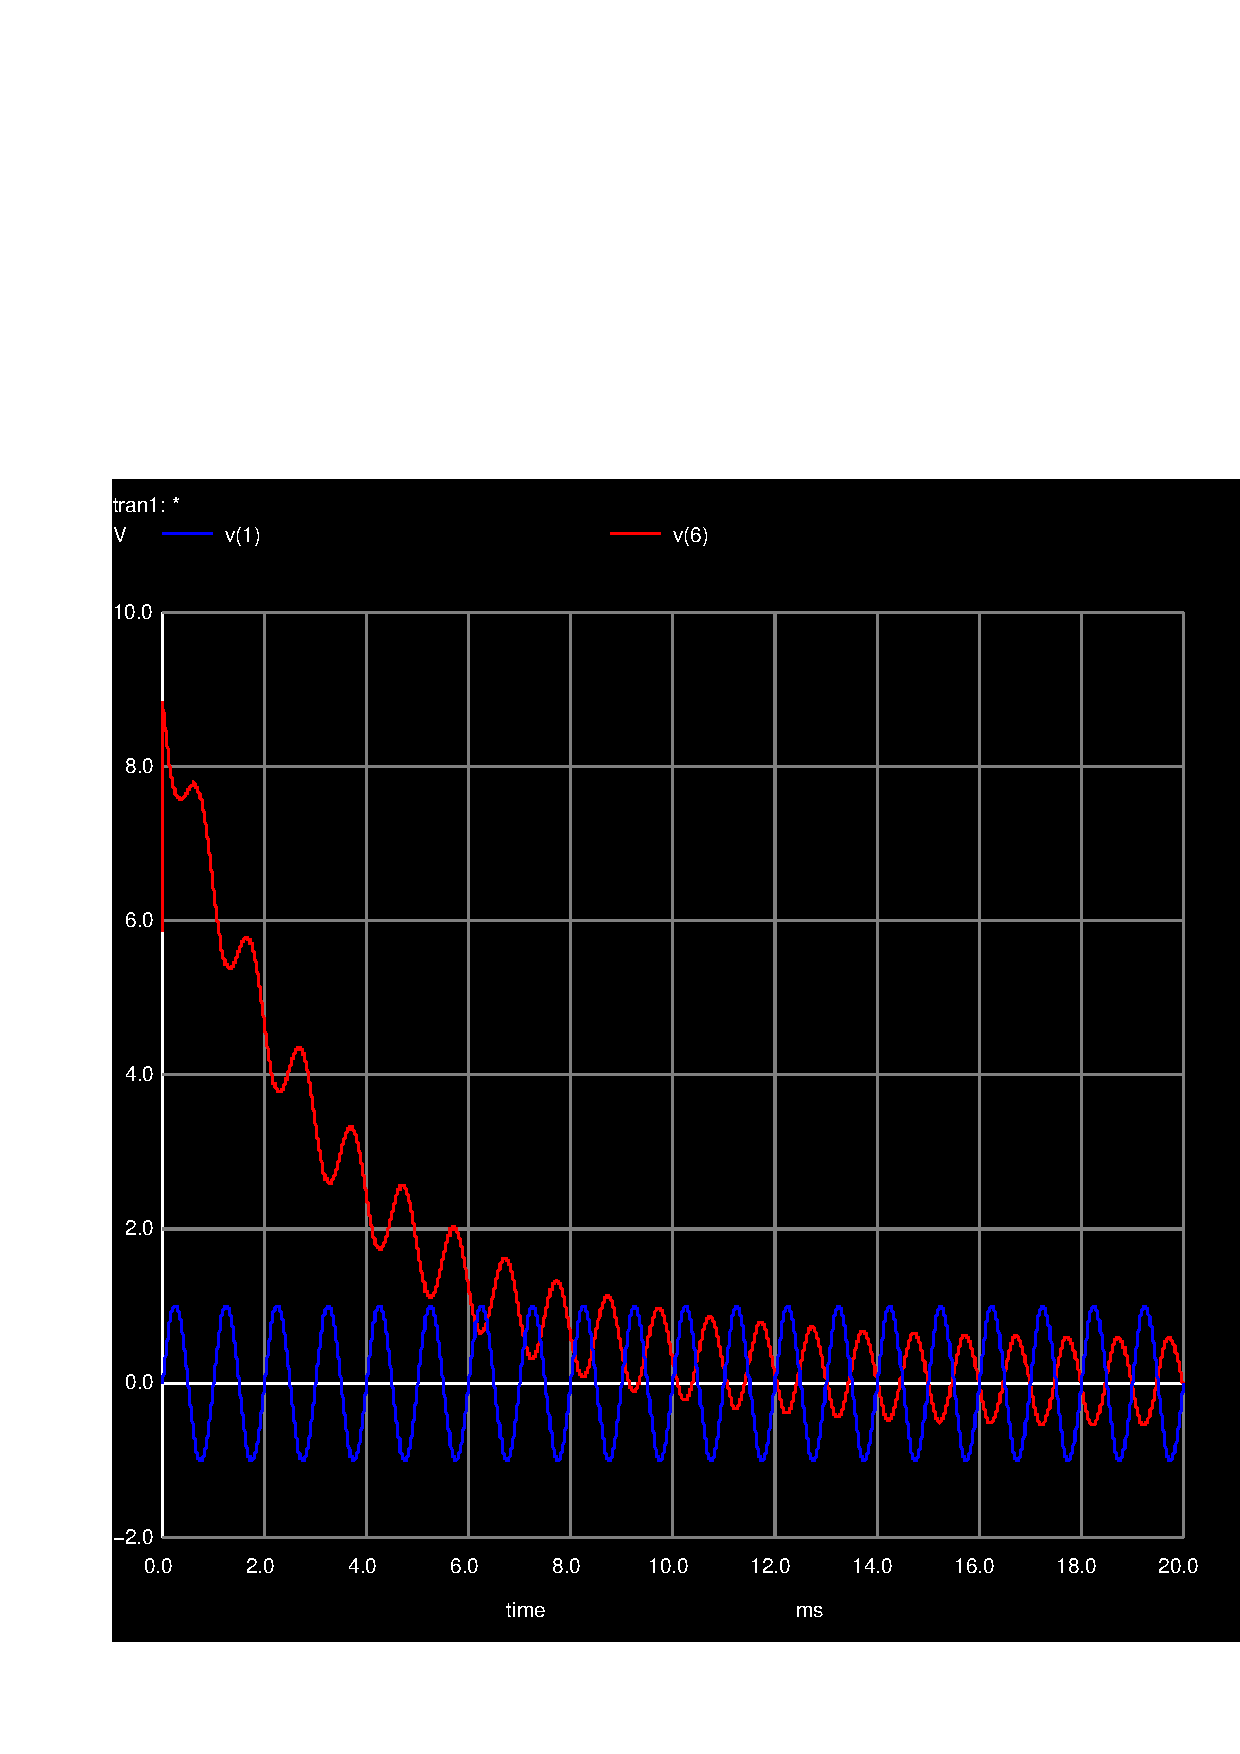
\includegraphics[width=\textwidth]{sim4.pdf}
\caption{Natural and forced response}
\label{fig:second}
\end{subfigure}
\end{figure}

When observing the graph obtained from the simulation  Ngspice, it is possible to conclude that, over the period of time considered, the voltage in the capacitor tends
to diminuish until its phase differs $\pi$ from the phase of the voltage source, such as in the graph obtained from the theorethical analysis in octave.

\subsection{Frequency Responses}

In this part of the assignment, an AC (Alternating Current) Analysis was conducted, in order to match the goal mentioned above. This type of analysis allows to study the frequency response of the circuit. For this, there is no frequency variation (steady-state analysis). After comparing the graphics showed below, it is clear to admit that the results in ngspice and octave match. Any minor difference may be explained by aproximation errors.

\subsubsection{Frequency Responses - Amplitude}

\begin{figure}[H] 
\centering
\begin{subfigure}{0.5\textwidth}
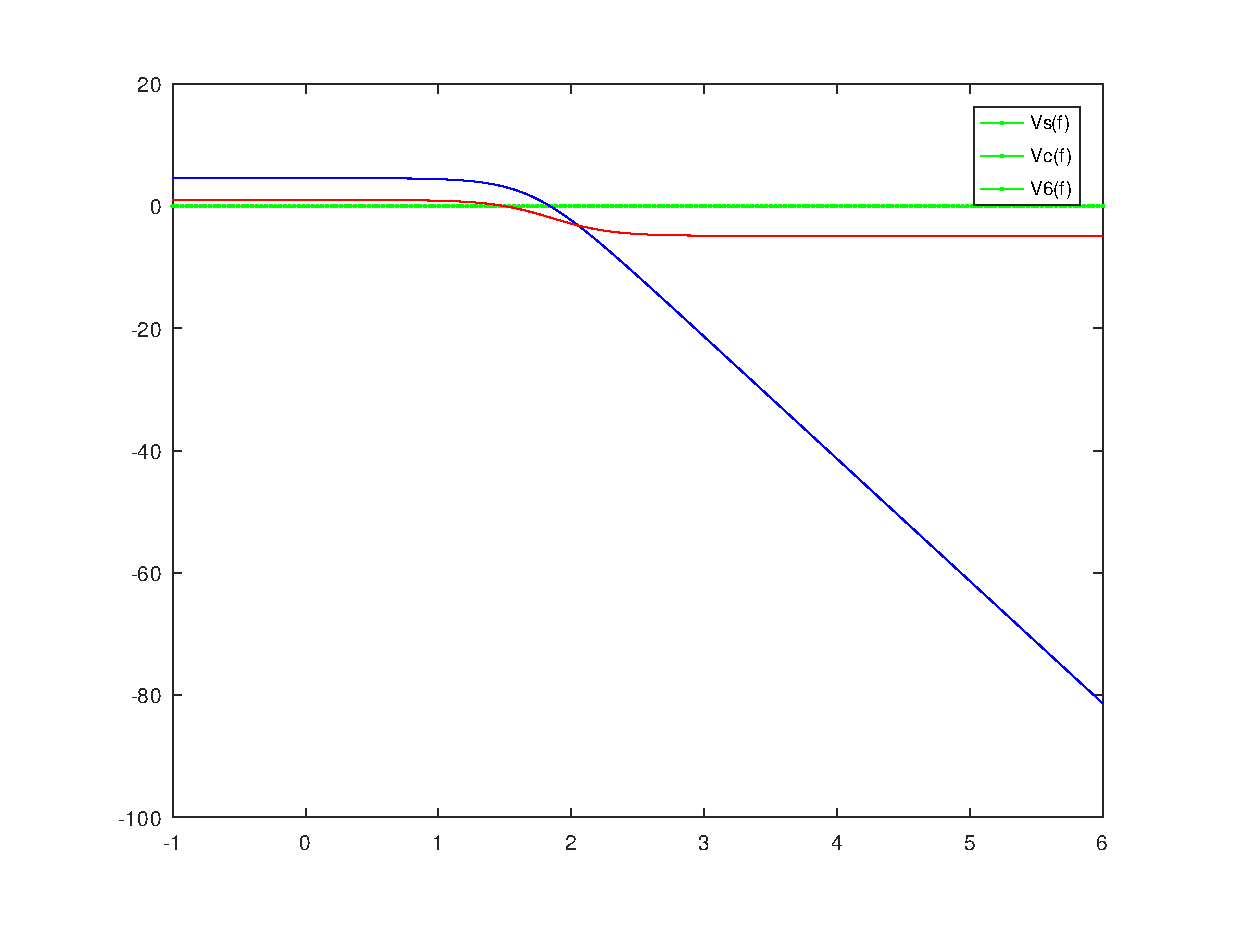
\includegraphics[width=\textwidth]{Amplitude.eps}
\caption{Amplitude (Octave)}
\label{fig:first}
\end{subfigure}
\begin{subfigure}{0.42\textwidth}
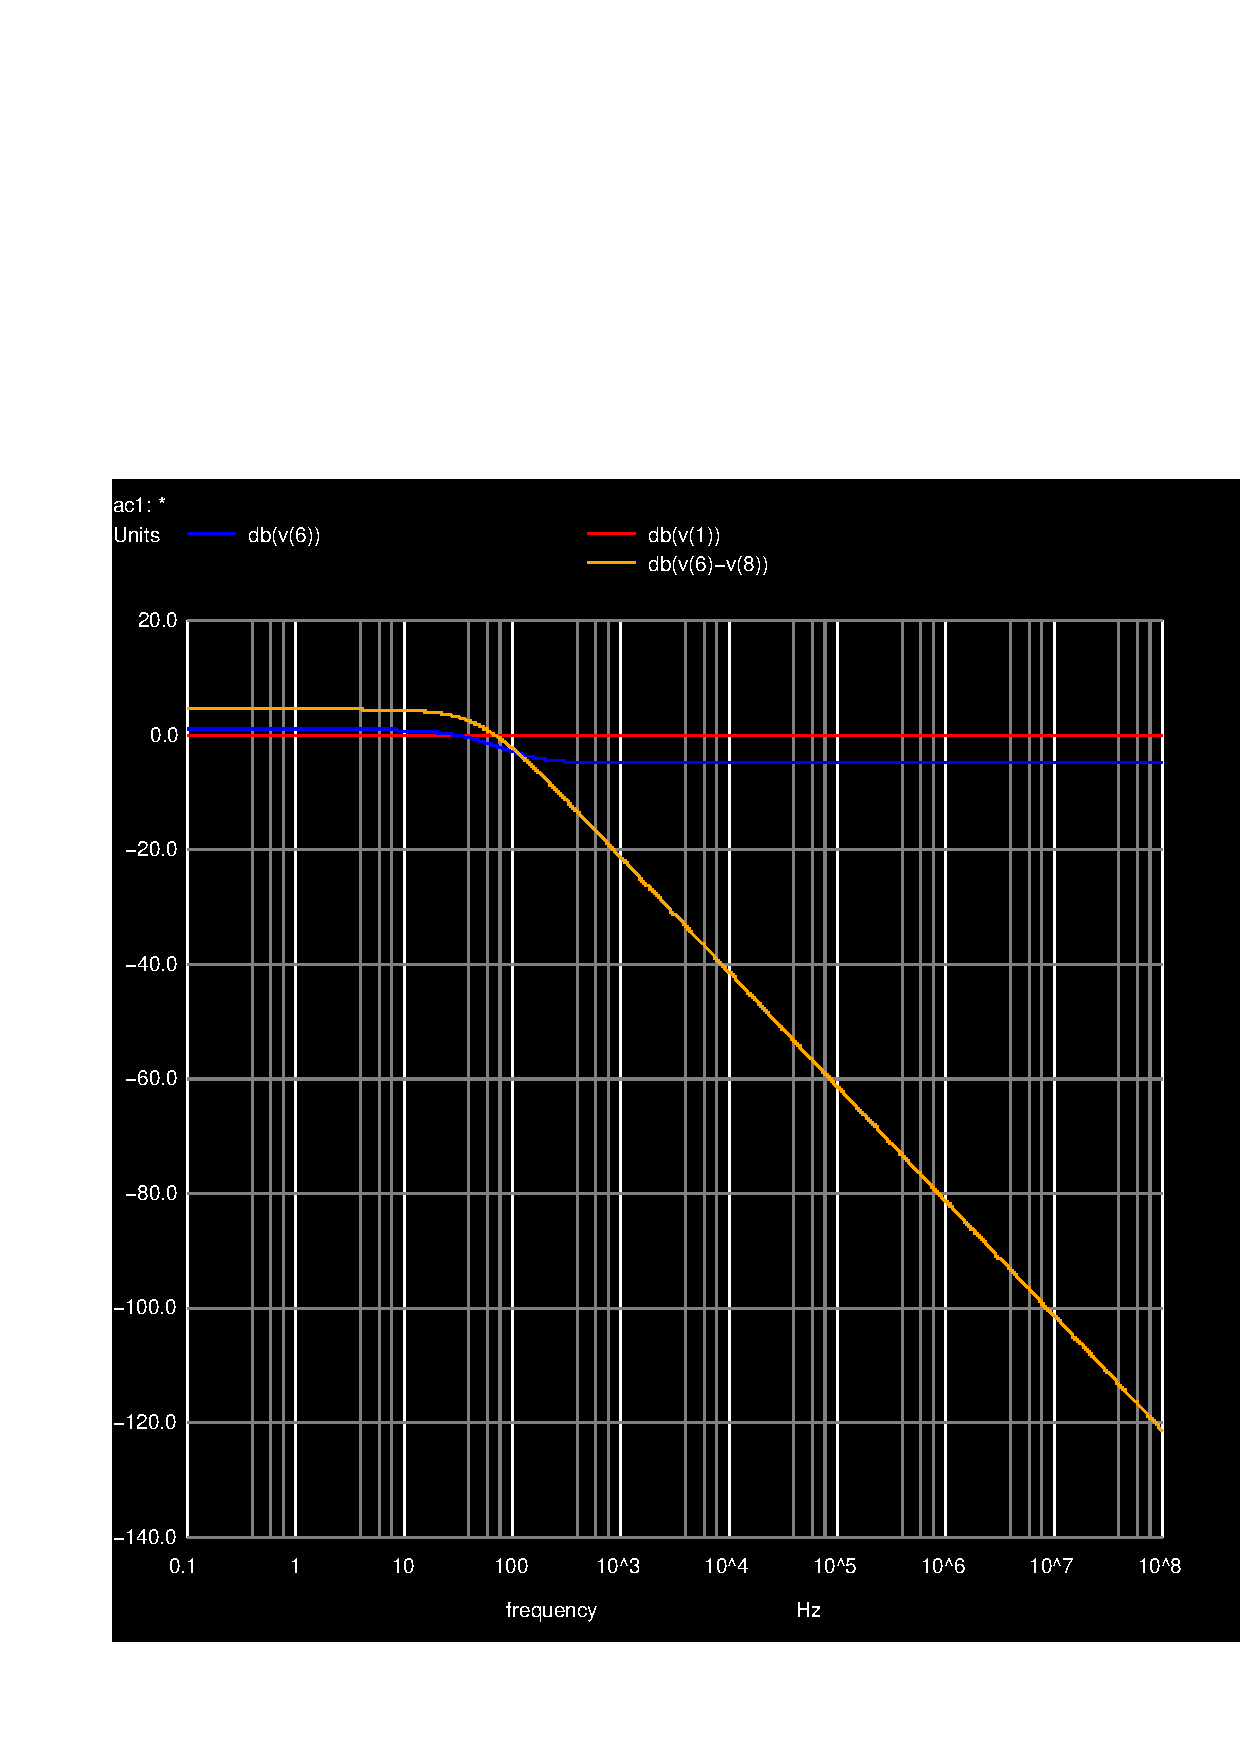
\includegraphics[width=\textwidth]{sim5_db.pdf}
\caption{Amplitude (NgSpice)}
\label{fig:second}
\end{subfigure}
\end{figure}

As expected, the results obtained from the ngspice simulation and the theorethical analysis in octave match.

\subsubsection{Frequency Responses - Phase}

\begin{figure}[H] 
\centering
\begin{subfigure}{0.5\textwidth}
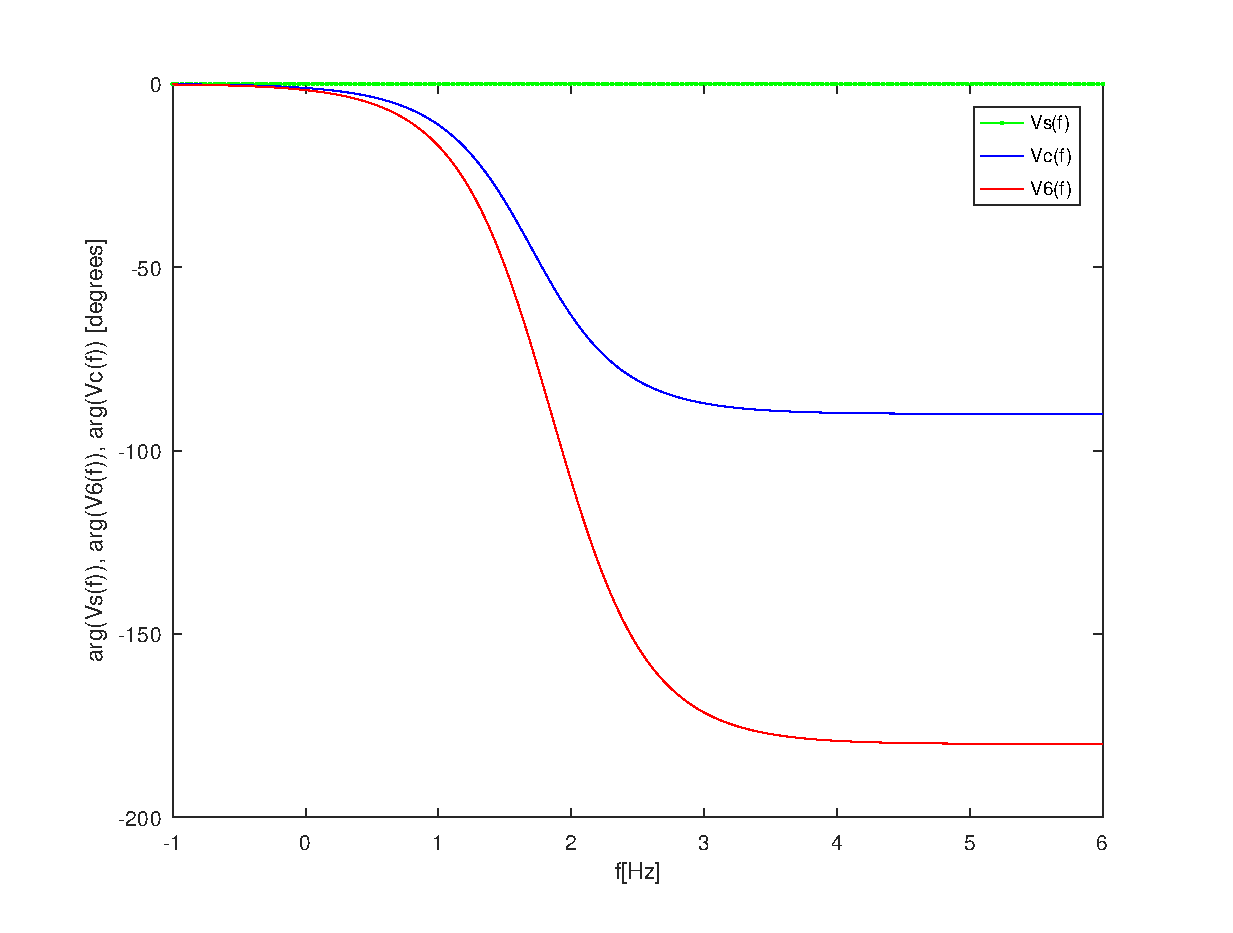
\includegraphics[width=8cm]{Arguments.eps}
\caption{Arguments (Octave)}
\label{fig:first}
\end{subfigure}
\begin{subfigure}{0.42\textwidth}
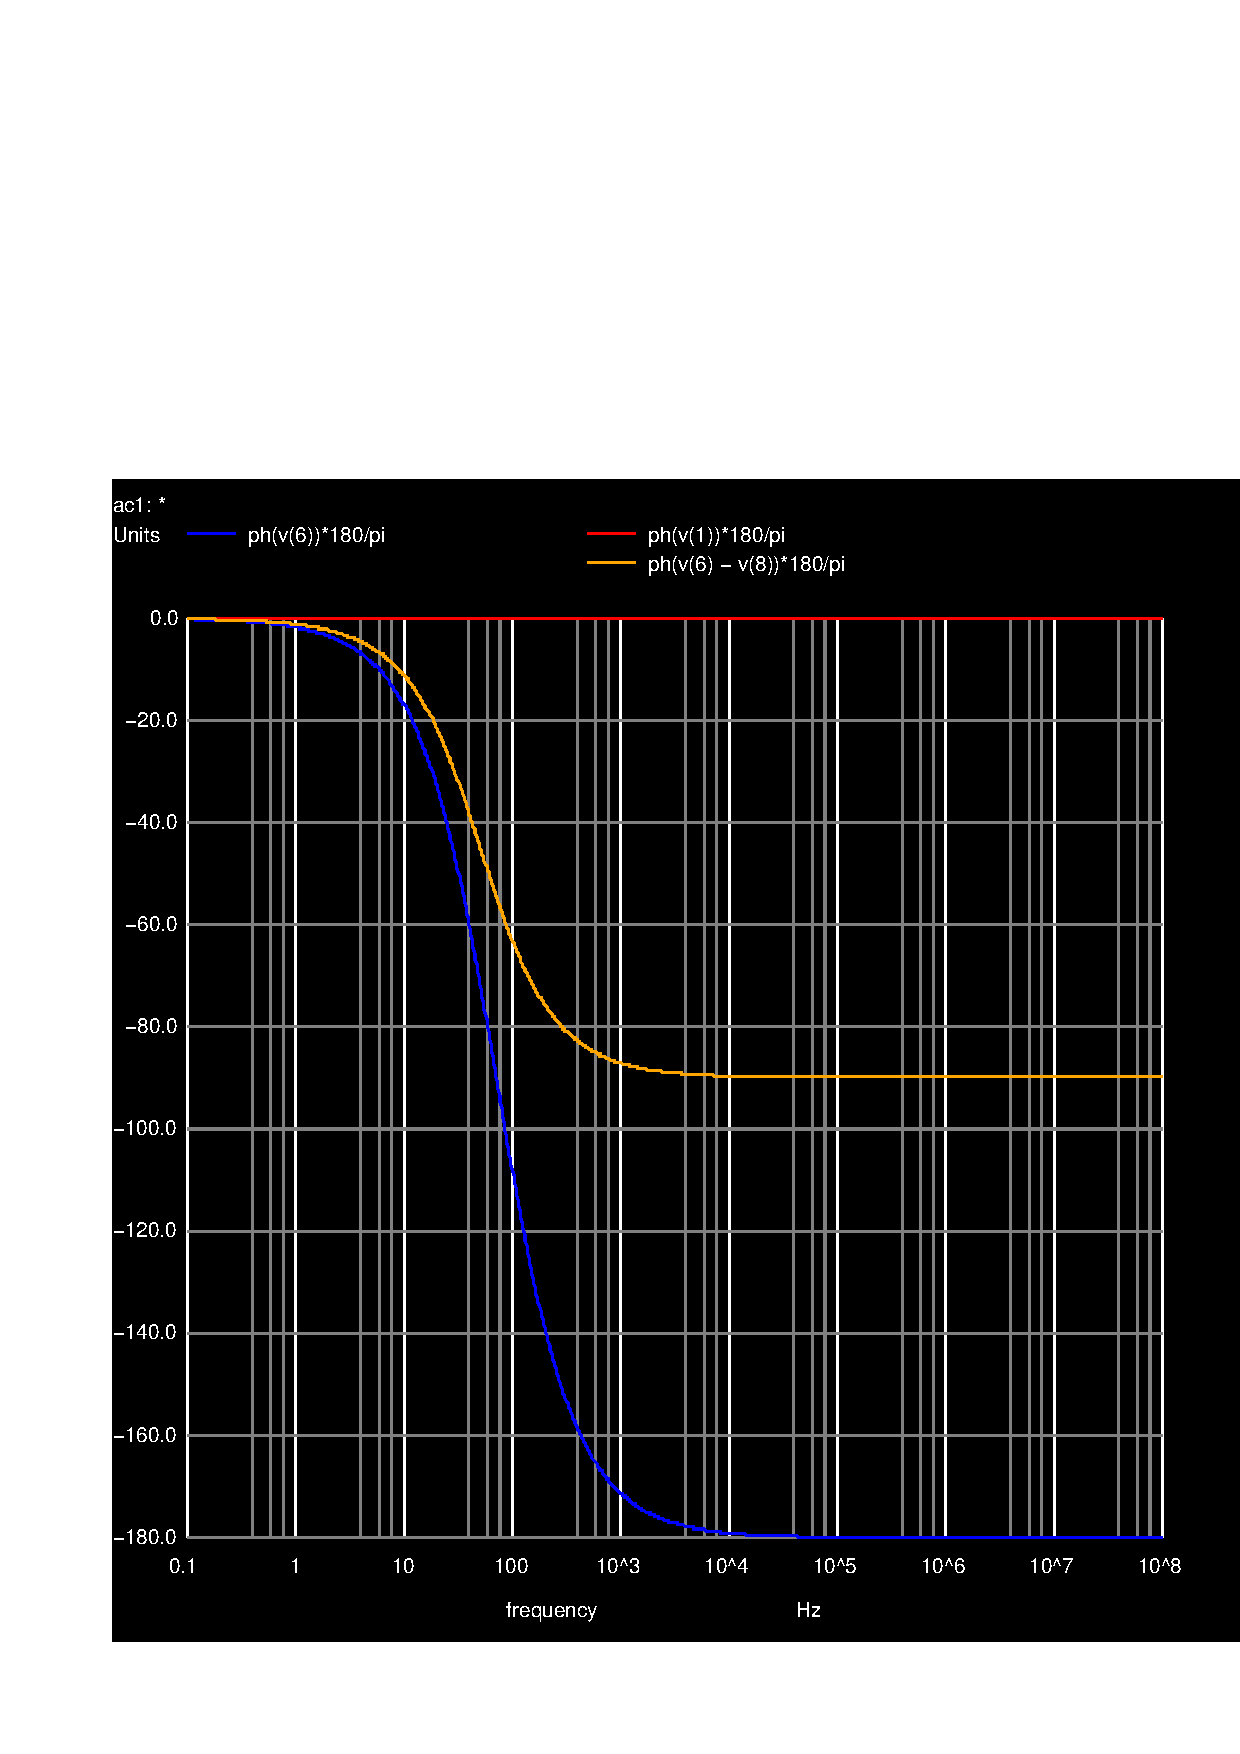
\includegraphics[width=8cm]{sim5_ph.pdf}
\caption{Arguments (NgSpice)}
\label{fig:second}
\end{subfigure}
\end{figure}

As expected, the results obtained from the ngspice simulation and the theorethical analysis in octave match.

